\chapter{إنتاج غذائنا}\label{ch:g6:producing-our-food}

لا شيء على مائدة فطورك وُجد في البرية. فقمح الخبز استُنبت وزُرع؛
\omterm{def:g2:animals-grow-up:born}{والحليب} جاء من قطعان تُربّى له؛ واللبن \emph{صنعه} من ذلك \omterm{def:g2:animals-grow-up:born}{الحليب}
ملايير من العمّال الأحياء الأصغر من أن يُروا. فالبشر يطعمون أنفسهم
بإدارة \omterm{def:g6:exploring-our-environment:components}{الكائنات الحية} --- بزراعتها، وتربيتها، وتشغيل بعض أصغرها.
وهذا الفصل جولة في مشغل الغذاء.

\section{الزراعة والتربية}

\begin{definition}[المحاصيل والماشية]\label{def:g6:producing-our-food:farming}
إنتاج الغذاء عند الإنسان يدير \omterm{def:g6:exploring-our-environment:components}{الكائنات الحية} عند طابقين من دورة
المادة:
\begin{itemize}
  \item \emph{زراعة المحاصيل}\index{محصول}: إدارة \omterm{def:g5:food-webs:roles}{المنتِجين} ---
        القمح، والبطاطا، والخضر، والفواكه --- من أجل مادتهم
        العضوية
        (\cref{prop:g6:plants-are-producers:produce})؛
  \item و\emph{تربية الماشية}\index{ماشية}: إدارة \omterm{def:g5:food-webs:roles}{المستهلِكين} ---
        الأبقار، والأغنام، والخنازير، والدجاج --- من أجل إنتاجهم
        للمادة (\cref{def:g6:matter-from-food:production}):
        \omterm{def:g2:animals-grow-up:born}{الحليب}، واللحم، \omterm{def:g2:animals-grow-up:born}{والبيض}، والصوف.
\end{itemize}
والمزارعون يديرون \omterm{def:g6:exploring-our-environment:conditions}{الشروط} التي ما ينفكّ هذا الكتاب يلقاها: معادن
\omterm{def:g6:decomposers-and-soil:soil}{التربة} للمحاصيل (\cref{rem:g4:what-plants-need:soil})، والعلف
\omterm{def:g1:animals-around-us:animal}{للحيوانات} --- أي دفتر \cref{pb:g6:matter-from-food:1} كله، مُدارًا
عن قصد.
\end{definition}

\begin{example}[ما حقل القمح]\label{ex:g6:producing-our-food:wheat}
حقل القمح \omterm{def:g6:exploring-our-environment:components}{بيئة} مُدارة
(\cref{prop:g5:people-and-nature:managed}) مضبوطة على منتِج واحد:
\omterm{def:g6:decomposers-and-soil:soil}{تربة} مُعاد تموينها ومفكَّكة لجذوره، وبذار موقوت على دفء
\cref{prop:g2:from-seed-to-plant:needs}، وأعشاب ضارّة --- وهي
مستوطنون منافسون من \cref{ch:g6:how-plants-spread} --- تُبعَد.
والحصاد هو مخزن \omterm{def:g2:from-seed-to-plant:seed}{بذور} \omterm{def:g1:plants-around-us:plant}{النبات}: الحبّ، وهو غداء مليون \omterm{def:g1:plants-around-us:plant}{نبتة} قمح لن
تُبذر أبدًا، محوَّلًا إلى المخابز.
\end{example}

\begin{remark}[كل غذاء مرحلة من دورة حياة]\label{rem:g6:producing-our-food:stage}
اقرأ أي غذاء قراءةً بيولوجية تجده عضوًا أو مرحلة من كائن ما:
فالحبّ والفول مخازن \omterm{def:g2:from-seed-to-plant:seed}{بذور}؛ والبطاطا \omterm{ex:g4:plants-without-seeds:bulbtuber}{درنات}؛ والتفاح \omterm{prop:g3:flowers-fruits-seeds:transform}{ثمار} مبنية لتُؤكل
(\cref{exo:g6:how-plants-spread:12})؛ \omterm{def:g2:animals-grow-up:born}{والحليب} عناية أمّ ثديية
(\cref{def:g2:animals-grow-up:born})؛ \omterm{def:g2:animals-grow-up:born}{والبيضة} حضّانة محزومة.
فإنتاج الغذاء فنّ إدارة دورات الحياة حتى تصل مؤنها إلى موائدنا.
\end{remark}

\section{القوة العاملة غير المرئية: غذاء تصنعه الميكروبات}

\begin{definition}[التخمّر]\label{def:g6:producing-our-food:fermentation}
بعض الأطعمة تُصنع بتشغيل كائنات حية أصغر من أن تُرى ---
\emph{ميكروبات}\index{ميكروب غذائي} --- على مادة خام. فتغذّيها
يحوّلها: ويسمى هذا التحويل
\emph{التخمّر}\index{تخمر}، وقد أداره البشر آلاف السنين، من قبل أن
يعرف أحد أن العمّال موجودون بزمن طويل.
\end{definition}

\begin{example}[الخبز يختمر]\label{ex:g6:producing-our-food:bread}
عجين الخبز الخام دقيق وماء --- مع \emph{الخميرة}\index{خميرة}،
وهي \omterm{def:g6:decomposers-and-soil:decomposers}{فطر} وحيد \omterm{def:g5:first-look-at-cells:cell}{الخلية}
(وقد لقيت \cref{rem:g5:first-look-at-cells:onecelled} حيوات كهذه).
فتتغذى \omterm{ex:g6:producing-our-food:bread}{الخميرة} على سكريات الدقيق وتطلق غازًا؛ وفقاقيع الغاز،
محبوسة في العجين المطاطي، تنفخه --- ويسميه الخبّاز الاختمار. ثم
تنهي حرارة الفرن نوبة العمّال وتثبّت عملهم: فثقوب اللبّ توقيع
\omterm{ex:g6:producing-our-food:bread}{الخميرة}.
\end{example}

\begin{omfigure}
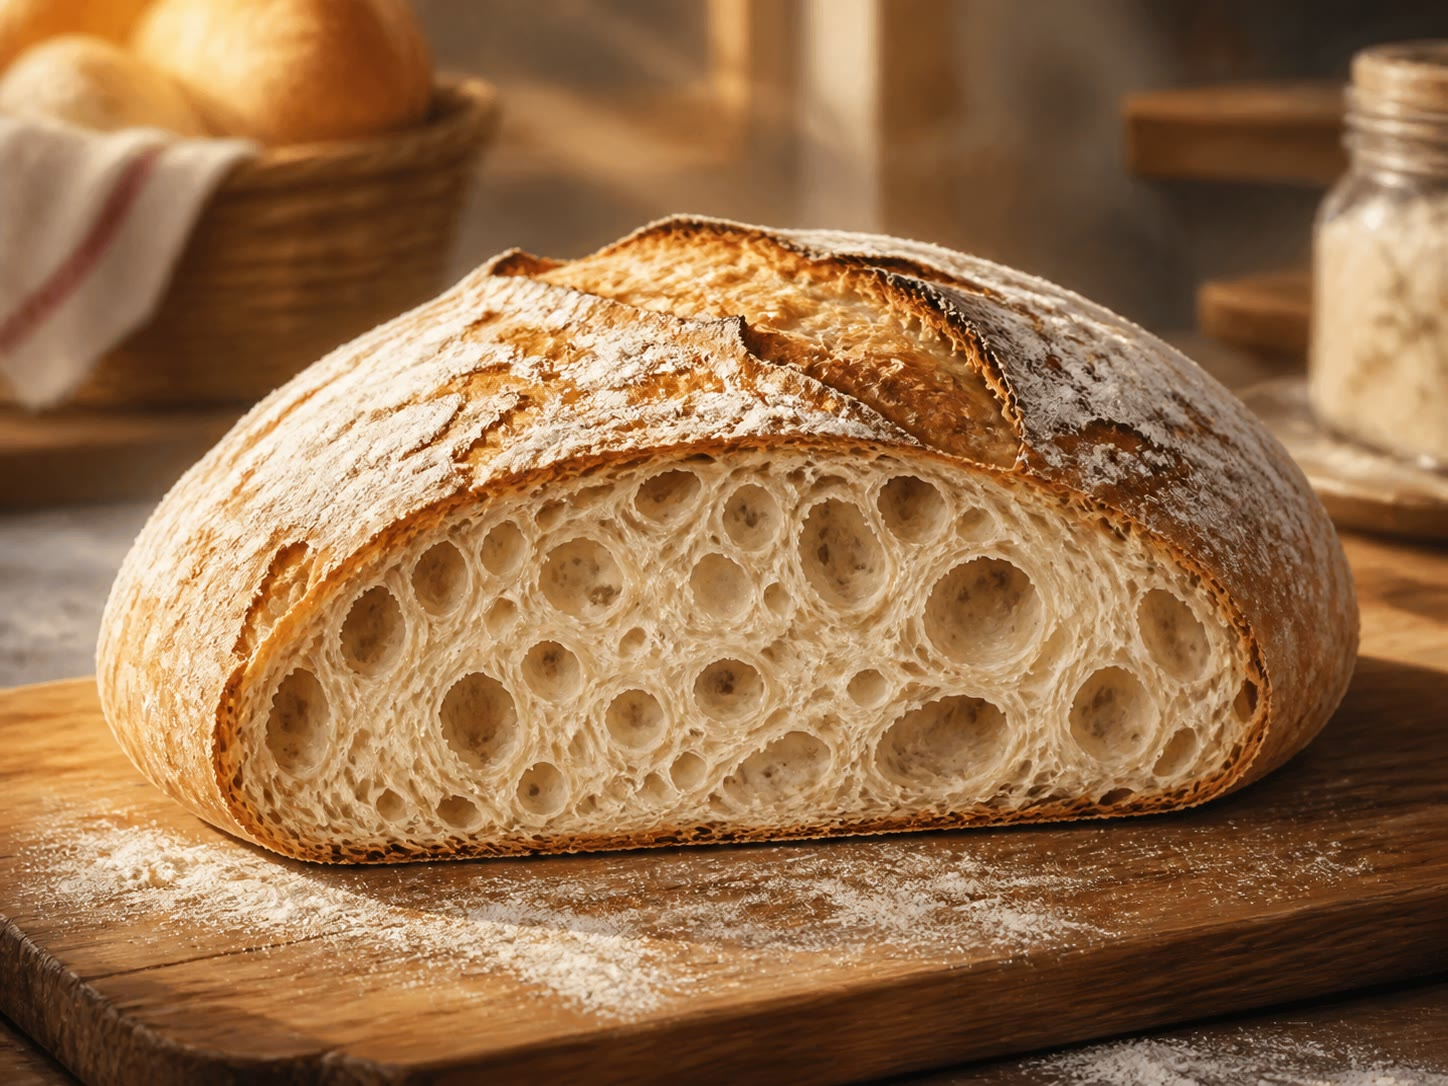
\includegraphics[width=0.58\linewidth]{images/book1/ai/g6-food-bread.jpg}

{\small توقيع القوة العاملة، مخبوزًا في مكانه: كل ثقب في اللبّ
فقاعة نفختها \omterm{ex:g6:producing-our-food:bread}{الخميرة}.}
\end{omfigure}

\begin{example}[الحليب يصير لبنًا وجبنًا]\label{ex:g6:producing-our-food:yogurt}
\omterm{def:g2:animals-grow-up:born}{الحليب} الدافئ المبذور \omterm{def:g6:producing-our-food:fermentation}{بالميكروبات} الصحيحة يثخن في ليلة فيصير لبنًا:
فالعمّال يتغذون على سكر \omterm{def:g2:animals-grow-up:born}{الحليب} ويطلقون حمضًا، والحمض يعقد \omterm{def:g2:animals-grow-up:born}{الحليب}
--- والحموضة الطازجة \emph{هي} ذلك الحمض. والجبن يبدأ بداية شبيهة
ثم يمضي أبعد: خثارة تُكبس وتُملّح وتُنضج شهورًا، \omterm{def:g6:producing-our-food:fermentation}{والميكروبات} تعمل
طول الإنضاج --- فثقوب الجبنة وقشرتها وقوة رائحتها سجلّ نوبتهم
الطويلة.
\end{example}

\begin{remark}[ميكروبات نافعة وأخرى ضارّة]\label{rem:g6:producing-our-food:goodbad}
علّمتنا \omterm{def:g1:healthy-habits:germs}{جراثيم} \cref{def:g1:healthy-habits:germs} الحذر من
\omterm{def:g6:producing-our-food:fermentation}{الميكروبات}؛ ويضيف هذا الفصل النصف الآخر: \omterm{def:g6:producing-our-food:fermentation}{فالميكروبات}
\emph{المختارة}، العاملة في \omterm{def:g6:exploring-our-environment:conditions}{شروط} \emph{مضبوطة}، من أقدم موظفينا ---
في الخبز، واللبن، والجبن، وبرميل الخلّ. والصنعة واحدة دائمًا: رحّب
بالعمّال المختارين، واحفظ شروطًا تناسبهم لا تناسب المفسدين. فالتمليح
والتبريد والتجفيف والطهي كلها طرق لمنع \omterm{def:g6:producing-our-food:fermentation}{الميكروبات} غير المرغوبة
شروطَها (و\cref{prop:g6:decomposers-and-soil:speed} تعمل على فخذ
لحم كما تعمل على كومة \omterm{def:g1:plants-around-us:parts}{أوراق} تمامًا).
\end{remark}

\section{من الحقل إلى المائدة بصدق}

\begin{proposition}[التكاليف على المائدة]\label{prop:g6:producing-our-food:costs}
كل صحن ناتج أرض وكائنات حية مُدارة، وهو يحمل حسابها:
\begin{itemize}
  \item فالأطعمة النباتية تصل على بعد طابق واحد من \omterm{def:g6:exploring-our-environment:conditions}{الضوء}؛ أما
        الأطعمة الحيوانية فتسلك طريق مستهلِك أولًا وتدفع رسم
        \cref{prop:g6:matter-from-food:losses}
        (\cref{exo:g6:matter-from-food:12})؛
  \item والإنتاج الدائم عليه أن يحفظ قواعد
        \cref{prop:g5:people-and-nature:lasting} الثلاث --- أطعم
        \omterm{def:g6:decomposers-and-soil:soil}{التربة}، وأبقِ المعينين، ولا تأخذ أسرع من التجدد؛
  \item والهدر ينقض ذلك كله: فالغذاء الملقى أنفق أرضه وماءه وعمله
        بلا أحد.
\end{itemize}
\end{proposition}
\admitted

\begin{method}[قراءة حكاية غذاء]\label{met:g6:producing-our-food:read}
لأي غذاء في المطبخ:
\begin{enumerate}
  \item سمِّ الكائن والعضو أو المرحلة التي هو إياها
        (\cref{rem:g6:producing-our-food:stage})؛
  \item وضعه على الدورة: أهو مادة منتِج، أم \omterm{def:g5:food-webs:roles}{منتج} مستهلِك، أم من
        صنع \omterm{def:g6:producing-our-food:fermentation}{الميكروبات}؟
  \item فإن كان من صنع \omterm{def:g6:producing-our-food:fermentation}{الميكروبات}، فسمِّ المادة الخام وما غيّره
        العمّال؛
  \item وتتبّعه إلى ورقته
        (\cref{met:g6:plants-are-producers:trace}) --- فالأثر ما
        زال ينتهي عند \omterm{def:g6:exploring-our-environment:conditions}{الضوء} دائمًا.
\end{enumerate}
\end{method}

\begin{example}[الطريقة على مائدة الفطور]\label{ex:g6:producing-our-food:breakfast}
اللبن بالطريقة: (1) \omterm{def:g2:animals-grow-up:born}{حليب} --- \omterm{def:g5:food-webs:roles}{منتج} عناية أمّ بقرة --- محوَّل؛ (2)
\omterm{def:g5:food-webs:roles}{منتج} مستهلِك، أنهته \omterm{def:g6:producing-our-food:fermentation}{الميكروبات}؛ (3) المادة الخام \omterm{def:g2:animals-grow-up:born}{حليب}، والعمّال
حمّضوه وعقدوه؛ (4) \omterm{def:g2:animals-grow-up:born}{الحليب} من البقرة، والبقرة من العشب، والعشب من
\omterm{def:g6:exploring-our-environment:conditions}{الضوء}. ثلاثة كائنات وقوة عاملة من الملايير، في قدح صغير واحد.
\end{example}

\section{تمارين}

\begin{exercise}[$\star$]\label{exo:g6:producing-our-food:1}
عرّف \omterm{def:g6:producing-our-food:farming}{زراعة المحاصيل} \omterm{def:g6:producing-our-food:farming}{وتربية الماشية}، مسمّيًا طابق دورة المادة الذي
تديره كل واحدة.
\end{exercise}

\begin{exercise}[$\star$]\label{exo:g6:producing-our-food:2}
لكل غذاء، سمِّ الكائن والعضو أو المرحلة: الحبّ، والبطاطا،
والتفاحة، \omterm{def:g2:animals-grow-up:born}{والحليب}، \omterm{def:g2:animals-grow-up:born}{والبيضة}.
\end{exercise}

\begin{exercise}[$\star$]\label{exo:g6:producing-our-food:3}
ما \omterm{def:g6:producing-our-food:fermentation}{التخمّر}؟ سمِّ طعامين مخمَّرين وموادّهما الخام.
\end{exercise}

\begin{exercise}[$\star$]\label{exo:g6:producing-our-food:4}
اذكر لماذا يختمر الخبز: العامل، وغذاؤه، وما يطلقه، وما يفعله
الفرن.
\end{exercise}

\begin{exercise}[$\star$]\label{exo:g6:producing-our-food:5}
ما الذي يعقد \omterm{def:g2:animals-grow-up:born}{الحليب} لبنًا، ومن أين تأتي الحموضة؟
\end{exercise}

\begin{exercise}[$\star$]\label{exo:g6:producing-our-food:6}
أعطِ ثلاث طرق لمنع \omterm{def:g6:producing-our-food:fermentation}{الميكروبات} غير المرغوبة شروطَها، من
\cref{rem:g6:producing-our-food:goodbad}.
\end{exercise}

\begin{exercise}[$\star\star$]\label{exo:g6:producing-our-food:7}
حقل القمح يدير كل حاجة من حاجات
\cref{prop:g4:what-plants-need:needs} عن قصد. اقرن كل حاجة بفعل
المزارع في \cref{ex:g6:producing-our-food:wheat}.
\end{exercise}

\begin{exercise}[$\star\star$]\label{exo:g6:producing-our-food:8}
طبّق \cref{met:g6:producing-our-food:read} على الجبن، خطوةً خطوة.
\end{exercise}

\begin{exercise}[$\star\star$]\label{exo:g6:producing-our-food:9}
لماذا يحفظ التبريد الغذاء --- ولماذا يبطّئ البرد نفسه كومة سماد؟
مبدأ واحد ومطبخان: سمِّه.
\end{exercise}

\begin{exercise}[$\star\star$]\label{exo:g6:producing-our-food:10}
وفّق بين \cref{def:g1:healthy-habits:germs} وهذا الفصل: كيف تكون
\omterm{def:g6:producing-our-food:fermentation}{الميكروبات} عدوّ غسل اليدين وقوة اللبن العاملة معًا؟
\end{exercise}

\begin{exercise}[$\star\star$]\label{exo:g6:producing-our-food:11}
مستعملًا \cref{prop:g6:producing-our-food:costs}، اشرح لماذا تهدر
شطيرة لحم ملقاة أكثر مما يهدره وزن مماثل من الخبز الملقى.
\end{exercise}

\begin{exercise}[$\star\star\star$]\label{exo:g6:producing-our-food:12}
أدار الخبّازون والمخمّرون \omterm{def:g6:producing-our-food:fermentation}{التخمّر} آلاف السنين من غير أن يعرفوا أن
\omterm{def:g6:producing-our-food:fermentation}{الميكروبات} موجودة. فما الذي أداروه حقًّا بمصطلحات
\cref{prop:g6:exploring-our-environment:decide} --- ولماذا نجحت
وصفاتهم مع ذلك؟
\end{exercise}

\section{مسألة: مخبز الصف}

\begin{problem}[{مسألة نهاية الأسبوع --- دفعة خبز واحدة، متتبَّعة
من البذرة إلى الشريحة}]\label{pb:g6:producing-our-food:1}
لمعرض المدرسة يخبز الصف خبزًا من الصفر --- ويُبقي دفتر أحيائه
مفتوحًا من زيارة حقل القمح في تموز إلى الأرغفة في تشرين الثاني.

\medskip\noindent\textbf{القسم الأول --- الحقل (تموز).}
\begin{enumerate}
  \item يعرض المزارع القمح الناضج: ``الحصاد غداء \omterm{def:g1:plants-around-us:plant}{النبتة}
        المحزوم.'' فكّك العبارة وفق \cref{def:g2:from-seed-to-plant:seed}
        --- ما كل حبة، ولمن حُزمت؟
  \item وفي \omterm{def:g1:plants-around-us:parts}{أوراق} مَن، وبأي مدخلات، صُنعت \omterm{def:g6:plants-are-producers:matter}{المادة العضوية} للحبّ؟
  \item لا يبذر المزارع في الخريف التالي إلا جزءًا من الحصاد
        ويبيع الباقي. سمِّ مصيرَي حبة القمح بلغة \omterm{def:g2:born-grow-die:cycle}{دورة الحياة}.
  \item تنال \omterm{def:g6:decomposers-and-soil:soil}{تربة} الحقل روثًا بعد الحصاد. فأي قاعدة ردّ هذه، وأي
        حاجة من حاجات \omterm{def:g1:plants-around-us:plant}{النبات} الخمس تخدم؟
\end{enumerate}

\medskip\noindent\textbf{القسم الثاني --- المخبز (تشرين الثاني).}
\begin{enumerate}[resume]
  \item يخلط الصف الدقيق والماء والملح \omterm{ex:g6:producing-our-food:bread}{والخميرة}، ويضع العجين في
        ركن دافئ. فلماذا دافئ؟ أجب عن \omterm{ex:g6:producing-our-food:bread}{الخميرة} كما تجيب عن أي عامل
        حي (والنمط في \cref{prop:g6:decomposers-and-soil:speed}).
  \item وبعد ساعة يكون العجين قد تضاعف. اشرح الاختمار: علام تغذت
        \omterm{ex:g6:producing-our-food:bread}{الخميرة}، وماذا أطلقت، وما الذي حبسه؟
  \item عجين فريق، نُسي عند نافذة باردة تهبّ منها الريح، لا يكاد
        يختمر. شخّص ذلك --- واذكر أي مقارنة اختبار منصف أجراها
        الفريقان من غير قصد.
  \item وفي الفرن يكفّ الرغيفان عن الاختمار ويثبتان. فماذا فعلت
        الحرارة بالقوة العاملة، وما الذي يبقى توقيعًا لها في
        اللبّ؟
\end{enumerate}

\medskip\noindent\textbf{القسم الثالث --- الحساب.}
\begin{enumerate}[resume]
  \item تتبّع الشريحة النهائية إلى \omterm{def:g6:exploring-our-environment:conditions}{الضوء}، حلقةً حلقة.
  \item يبيع المعرض أيضًا شطائر زبدة وشطائر لحم. رتّب الشريحة
        والزبدة واللحم بحسب الطوابق التي سلكتها مادتها، واذكر
        أيها دفع أكبر رسم في
        \cref{prop:g6:matter-from-food:losses}.
  \item العجين غير المباع يُسمَّد ولا يُرمى. تابع مادته العضوية
        دورةً أخرى في الدائرة --- من يأخذها، وإلى ماذا؟
  \item أغلق الدفتر بجملة واحدة تحوي: المنتِج، والمستهلِك (إن
        وُجد)، والقوة العاملة الميكروبية، \omterm{def:g6:exploring-our-environment:conditions}{والضوء}.
\end{enumerate}
\end{problem}
